\documentclass[12pt, a4paper]{AnantDocumentation}

\title{ECE F311 - Communication Systems \\ Emona Lab Report}
\author{Pranav Chandra N. V. \\ 2023AAPS0013P}
\date{28th September, 2025}
\backgroundsetup{
	contents = ""
}

\usepackage[T1]{fontenc}
\usepackage{listings}
\lstset{
	backgroundcolor=\color{white},
	basicstyle=\ttfamily\small,
	breaklines=true,
	frame=single,
	numbers=left,
	numberstyle=\tiny,
	keywordstyle=\color{blue},
	commentstyle=\color{gray},
	stringstyle=\color{red},
	showstringspaces=false
}

\begin{document}
\maketitle

\section{Introduction and Objective}
To study the generation and demodulation of a Single Sideband (SSB) signal using an analog/digital trainer kit (EMONA Telecoms Trainer 101) and verify the results on a digital storage oscilloscope (Keysight DSO1014A).

\section{Basic Theory}
With Amplitude Modulation (AM), the carrier signal $c(t) = A_c \cos(2\pi f_c t)$ is modulated by a message signal $m(t)$ to produce the AM signal:
\begin{equation}
	AM(t) = A_c \left[1 + k_a m(t)\right] \cos(2\pi f_c t)
\end{equation}
This carrier multiplication creates a double sideband signal centered around the carrier. To make this better, we shift to DSB-SC.

DSB-SC is Double Side Band Suppressed Carrier modulation. In DSB-SC, the carrier is completely suppressed, and only the two sidebands are transmitted. The DSB-SC signal can be represented as:
\begin{equation}
	DSB(t) = m(t) \cos(2\pi f_c t)
\end{equation}
One thing we can see about this is that both the upper and lower sidebands are present, which means that the signal is transmitted in two bands. To make this better, we shift to SSB.

Single Side Band Modulation (SSB) is a refinement of DSB-SC where only one sideband (either upper or lower) is transmitted, and the other sideband is suppressed. The SSB signal can be represented as:
\begin{equation}
	SSB(t) = m(t) \cos(2\pi f_c t) \pm \hat{m}(t) \sin(2\pi f_c t)
\end{equation}
SSB reduces the required bandwidth by half compared to DSB-SC and improves power efficiency since only one sideband is transmitted.

\section{Experimental Setup}
The experimental setup used the \textbf{EMONA Telecoms Trainer 101} kit with the following steps:
\begin{enumerate}
	\item Message Signal Generation: A low-frequency message signal was generated and it's $90$ phase-shifted version was also created.
		\begin{figure}[h!]
			\centering
			\begin{subfigure}{0.45\textwidth}
				\centering
				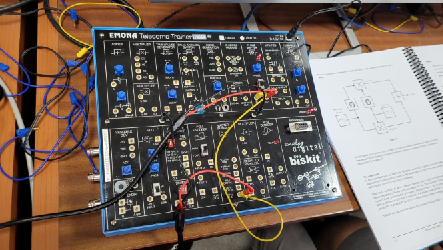
\includegraphics[width=\textwidth]{images/message-signal-gen-setup.png}
				\caption{Experimental Setup}
				\label{fig:message-signal-gen-setup}
			\end{subfigure}
			\hfill
			\begin{subfigure}{0.45\textwidth}
				\centering
				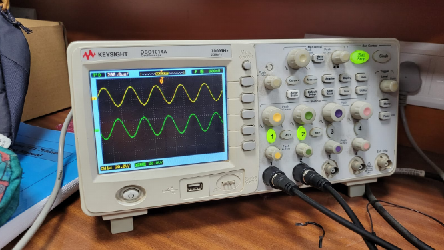
\includegraphics[width=\textwidth]{images/shifted-message-signal.png}
				\caption{DSO Output of Signals}
				\label{fig:shifted-message-signal}
			\end{subfigure}
			\caption{Message Signal Generation}
			\label{fig:message-signal-gen}
		\end{figure}
	\item Multiplication with a Carrier Signal: The original signal is multiplied by the cos signal of some frequency, while the hilbert transformed signal is multiplied by a sine signal of the same frequency.
		\begin{figure}[h!]
			\centering
			\begin{subfigure}{0.45\textwidth}
				\centering
				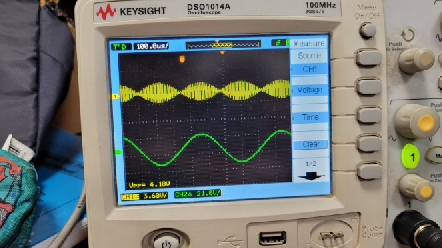
\includegraphics[width=\textwidth]{images/message-plus-carrier.png}
				\caption{$m(t) \times \cos(2 \pi f_c t)$}
				\label{fig:message-plus-carrier}
			\end{subfigure}
			\hfill
			\begin{subfigure}{0.45\textwidth}
				\centering
				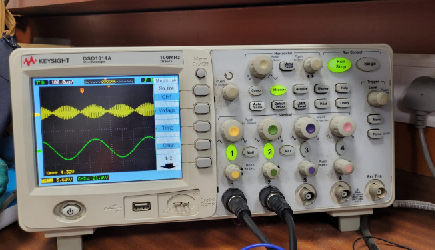
\includegraphics[width=\textwidth]{images/hilbert-plus-carrier.png}
				\caption{$\hat{m}(t) \times \sin(2 \pi f_c t)$}
				\label{fig:hilbert-plus-carrier}
			\end{subfigure}
			\caption{Signals Multiplied by their Carrier Signals}
			\label{fig:multiplier}
		\end{figure}
		\newpage
	\item SSB Signal Generation: The two signals from the previous step are added to generate the SSB signal.
		\begin{figure}[h!]
			\centering
			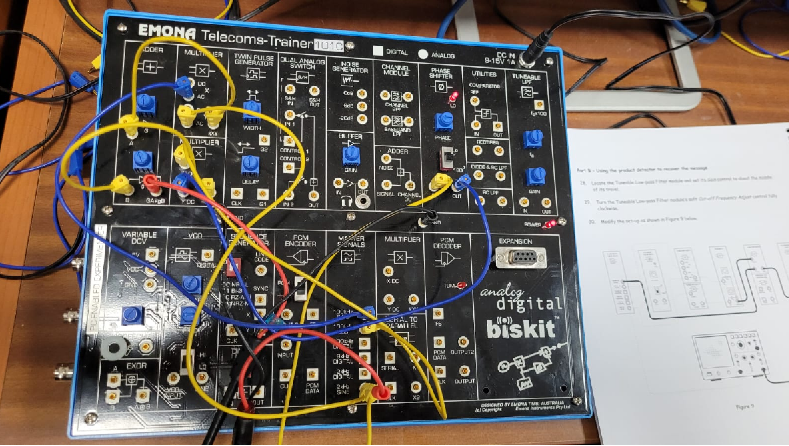
\includegraphics[width=0.7\textwidth]{images/ssb-generation-setup.png}
			\caption{Hardware Setup for SSB Generation}
			\label{fig:ssb-generation-hardware}
		\end{figure}
		
		\begin{figure}[h!]
			\centering
			\begin{subfigure}{0.45\textwidth}
				\centering
				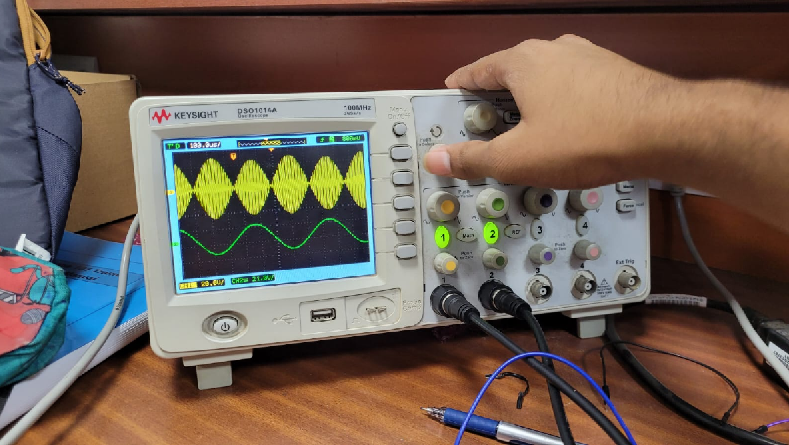
\includegraphics[width=\textwidth]{images/dsb-sc-signal.png}
				\caption{DSB-SC Reference SIgnal}
				\label{fig:dsb-sc-signal}
			\end{subfigure}
			\hfill
			\begin{subfigure}{0.45\textwidth}
				\centering
				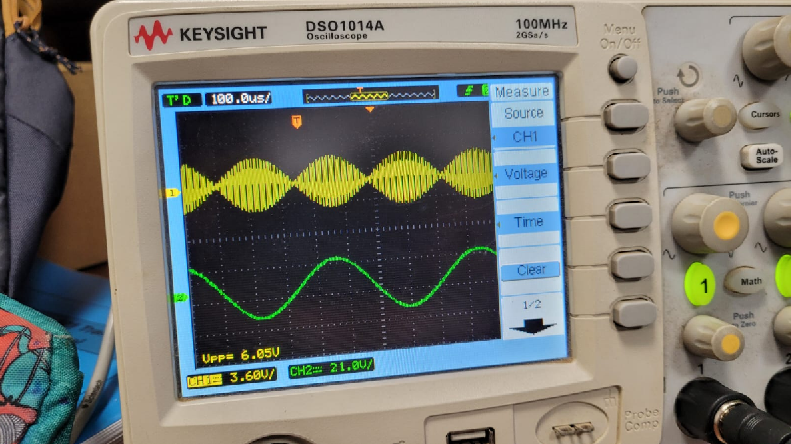
\includegraphics[width=\textwidth]{images/final-ssb-signal.png}
				\caption{Final SSB Signal}
				\label{fig:ssb-signal}
			\end{subfigure}
			\caption{SSB Signal Generation}
			\label{fig:ssb-generation}
		\end{figure}
	\item SSB Signal Demodulation: The SSB signal is demodulated using a product detector by multiplying it with a carrier signal of the same frequency and then passing it through a low-pass filter.
		\begin{figure}[h!]
			\centering
			\begin{subfigure}{0.45\textwidth}
				\centering
				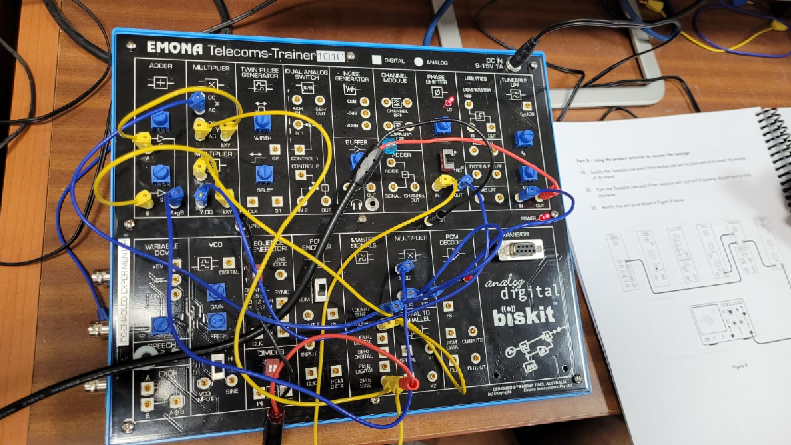
\includegraphics[width=\textwidth]{images/demodulation-setup.png}
				\caption{Demodulation Hardware Setup}
				\label{fig:demodulation-setup}
			\end{subfigure}
			\hfill
			\begin{subfigure}{0.45\textwidth}
				\centering
				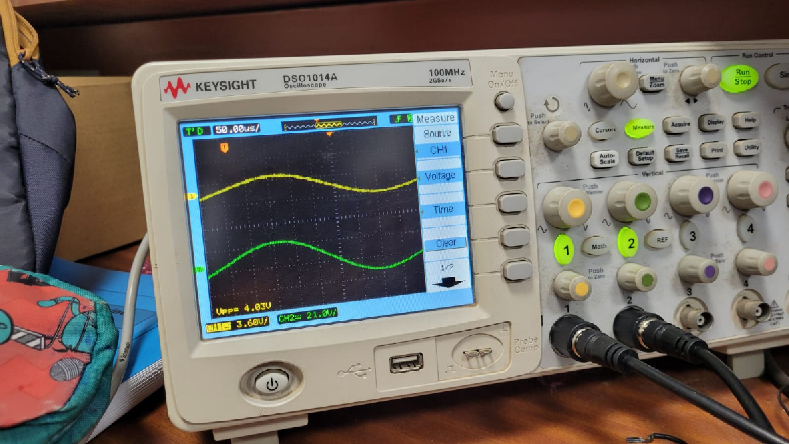
\includegraphics[width=\textwidth]{images/demodulated-signal.png}
				\caption{Demodulated SSB Signl (Top) and Original Signal (Bottom)}
				\label{fig:demodulated-ssb-signal}
			\end{subfigure}
			\caption{SSB Signal Demodulation}
			\label{fig:ssb-demodulation}
		\end{figure}

\end{enumerate}
\end{document}
